\documentclass[11pt]{article}
\usepackage{enumitem}
\usepackage{listings}
\usepackage[listings]{tcolorbox}
\usepackage{tikz}
\usepackage{url}

%\usepackage{algorithm2e}
\usetikzlibrary{arrows,automata,shapes}
\tikzstyle{block} = [rectangle, draw, fill=blue!20, 
    text width=5em, text centered, rounded corners, minimum height=2em]
\tikzstyle{bt} = [rectangle, draw, fill=blue!20, 
    text width=1em, text centered, rounded corners, minimum height=2em]

\lstset{ %
language=Java,
basicstyle=\ttfamily,commentstyle=\scriptsize\itshape,showstringspaces=false,breaklines=true,numbers=left}
\newtcbinputlisting{\codelisting}[3][]{
    extrude left by=1em,
    extrude right by=2em,
    listing file={#3},
    fonttitle=\bfseries,
    listing options={basicstyle=\ttfamily\footnotesize,numbers=left,language=Java,#1},
    listing only,
    hbox,
}


\newtheorem{defn}{Definition}
\newtheorem{crit}{Criterion}

\newcommand{\handout}[5]{
  \noindent
  \begin{center}
  \framebox{
    \vbox{
      \hbox to 5.78in { {\bf Software Testing, Quality Assurance and Maintenance } \hfill #2 }
      \vspace{4mm}
      \hbox to 5.78in { {\Large \hfill #5  \hfill} }
      \vspace{2mm}
      \hbox to 5.78in { {\em #3 \hfill #4} }
    }
  }
  \end{center}
  \vspace*{4mm}
}

\newcommand{\lecture}[4]{\handout{#1}{#2}{#3}{#4}{Lecture #1}}
\topmargin 0pt
\advance \topmargin by -\headheight
\advance \topmargin by -\headsep
\textheight 8.9in
\oddsidemargin 0pt
\evensidemargin \oddsidemargin
\marginparwidth 0.5in
\textwidth 6.5in

\parindent 0in
\parskip 1.5ex
%\renewcommand{\baselinestretch}{1.25}

\begin{document}

\lecture{2 --- January 8, 2025}{Winter 2025}{Patrick Lam}{version 1}

\section*{Why Tests?}
Let's start by talking about what test suites can do for you (as a developer).

Reference: Kat Busch. ``A beginner's guide to automated testing.'' \\
\url{https://hackernoon.com/treat-yourself-e55a7c522f71}

Back to the situation in Lecture 1. You write some new code, and want some assurance that it works.
Passing code review at Dropbox at the time required tests along with the code.

``Lo and behold, I soon needed to fix a small bug.'' But, of course, 
it's easy to introduce even more bugs when fixing something.
Fortunately, she had some tests.

\begin{quote}
I ran the tests. Within a few seconds, I knew that everything still worked! Not just a single code path (as in a manual test), but all code paths for which I’d written tests! It was magical. It was so much faster than my manual testing. And I knew I didn’t forget to test any edge cases, since they were all still covered in the automated tests.
\end{quote}

Not writing tests is incurring technical debt. You'll pay for it
later, when you have to maintain the code. Having tests
allows you to move faster later, without worrying about breaking your
code.

\begin{quote}
If your code is still in the codebase a year (or five) after you've
committed it and there are no tests for it, bugs will creep in and
nobody will notice for a long time.
\end{quote}

Writing tests is like eating your vegetables. It'll enable your code to go big and strong.

\begin{quote}
{\bf If it matters that the code works you should write a test for it.} There is no other way you can guarantee it will work.
\end{quote}

(We'll look at other ways in this course, but tests are the state of the industry.)

\section*{Exploratory Testing}
\vspace*{-1em}

Exploratory testing is usually (but not always) carried out by
dedicated testers. In that sense, it's somewhat different from the
other testing activities in this course, which are more
developer-focussed---our usual goal is learning, as developers, how to
deploy better automated test suites for our software. Hallway
usability testing, though, is an application of exploratory testing.
Furthermore, the dedicated QA function is important, and we should
learn about how it works.

\paragraph{Resources.} James Bach has an introduction 
to exploratory testing:\\[-2em]
{\scriptsize
\begin{itemize}[noitemsep]
\item \url{https://www.satisfice.com/exploratory-testing}
\end{itemize}
}
There is an exhaustive set of notes on exploratory testing by Cem Kaner:\\[-2em]
{\scriptsize
\begin{itemize}
\item \url{https://www.kaner.com/pdfs/QAIExploring.pdf}
\end{itemize}
}

\begin{quote}
``Exploratory testing is simultaneous learning, test design, and test execution.''
\end{quote}
Contrast this to scripted testing: test design
happens ahead of time and then test execution happens (repeatedly)
throughout the product's development cycle. When we think of
dedicated QA teams, we think they are manually executing scripted
tests. In 2025, that is not an effective use of staff.

There is a continuum between scripted testing and exploratory testing.
Good exploratory testing may use prepared scripts for certain tasks.

\paragraph{Scenarios where Exploratory Testing Excels.} (from Bach's article)
\begin{itemize}[noitemsep]
\item providing rapid feedback on new product/feature;
\item learning product quickly;
\item diversifying testing beyond scripts;
\item finding single most important bug in shortest time;
\item independent investigation of another tester's work;
\item investigating and isolating a particular defect;
\item investigate status of a particular risk to evaluate need for scripted tests.
\end{itemize}

\paragraph{Exploratory Testing Process.} Exploratory testing should not be
randomly bumbling around (we can call that ``ad hoc testing'')---the random
approach finds bugs but isn't the most efficient at giving you an idea of how well
the software works.

\begin{itemize}[noitemsep]
\item Start with a charter for your testing activity, e.g. ``Explore and analyze the product elements of the software.'' 
These charters should be somewhat ambiguous.
\item Decide what area of the software to test.
\item Design a test (informally).
\item Execute the test; log bugs.
\item Repeat.
\end{itemize}
Exploratory testing shouldn't produce an exhaustive set of notes. Good testers will
be able to reproduce the bugs that they encounter during their testing from brief notes.
Taking full notes takes too long.

The output from exploratory testing is at least a set of bug
reports. It may also include test notes, which include overall
impressions and a summary of the test strategy/thought
process. Artifacts such as test data or test materials are also both
inputs and outputs from exploratory testing.

\paragraph{Primary vs contributing tasks.}
One way to classify tasks that software can do (or, in other words, its features) is
\emph{primary} vs \emph{contributing}. A \emph{primary} task is core functionality of
the system; it's something that you would say ``You Had One Job!'' about. As examples,
text editors must be able to load text files, add text, and save the text files.
On the other hand, \emph{contributing} tasks are secondary. A macro system for a text
editor would be a contributing task. Being able to read email in your editor is
definitely a contributing task. Sometimes it's not black-and-white. Spell-check
can go either way.

\vspace*{-1em}
\section*{In-class exercise: Exploratory testing of WaterlooWorks.}
\vspace*{-1em} We will try out exploratory testing with
WaterlooWorks. I believe that all non-exchange students here should have
access to the system, although there may be no jobs visible right now.

The charter will be ``Explore the overall functionality of WaterlooWorks''. Summarize
in one or two sentences what the purpose of WaterlooWorks is. Identify the tasks that
WaterlooWorks should be able to do and classify them as primary or contributing. Identify
areas of potential instability. Test each function and record results (bugs).

Of course, don't do things that have actual effects. Usually, testers would have access 
to a development server and could test those areas more aggressively. But we are working
with production systems here.

\section*{Regression Testing}

Regression testing refers to any software testing that uncovers errors by retesting the modified program (Wikipedia). This form of testing often refers to comprehensive sets of test cases to detect regressions:
\begin{itemize}[noitemsep]
\item of bug fixes that a developer has proposed.
\item of related and unrelated other features that have been added.
\end{itemize}

Regression testing usually refers to system level (integration level) testing that runs the entire process.

\subsection*{Attributes of Regression Tests}

Regression tests usually have the following attributes:

\begin{itemize}[noitemsep]
\item \textbf{Automated}: no real reason to have manual regression tests.
\item \textbf{Appropriately Sized}: too small and bugs will be missed. Too large and they will take a long time to run. Optimally, we want to run tests continuously.
\item \textbf{Up-to-date}: ensure that tests are valid for the version of program being tested.

\end{itemize}

\subsection*{Automating Regression Tests}

Regression tests often have a low yield in terms of finding bugs (and are boring to run). Automation is key.

\textbf{Input}

If the input is from a file, regression tests are easy to run (but should still be automatically triggered on a regular interval). There may still be a problem with validating output. We can also create special mocks that can take input from a file or other sources (e.g. scripting engines). 

For UIs, the standard approach is to capture and replay events. This approach can be fragile! For example, tests may fail based on window placement or whitespace. For web applications, there is capture and replay for HTTP using Selenium (see L02-extra notes). Mozilla has a project named Marionette\footnote{\url{https://developer.mozilla.org/en-US/docs/Mozilla/QA/Marionette}} that is used to test Firefox and Thunderbird; it is like Selenium but also works on Chrome elements. 

\textbf{Output}

Verifying output can be hard!! Problems can arise from issues such as resolution, whitespace, window placement etc. 

\textbf{Mozilla Case Study\footnote{\url{http://robert.ocallahan.org/2005/03/visual-regression-tests_04.html}}}

The case study presents an approach to testing Gecko based applications. Gecko is the layout engine for Mozilla applications like Firefox and Thunderbird. 

In the past, a frame tree with coordinates for all UI elements was created and manual testers performed tests. Not optimal! The new approach was to capture screenshots after test cases and compare them with the expected screenshot. There were a few problems with the approach due to nondeterminism: 

\begin{itemize}[noitemsep]
\item Animated images: no way to ensure tests would function with animated images.
\item Font Hinting: the same character would appear slightly differently after each run of the application.
\item Other bugs: resolution problems, minor changes in layout etc.
\end{itemize}

The problem was ``really hellish'' and the partial solution was to enable logging in the application. The logs would essentially be compared with expected logs. This became very ugly given 1300 or so test cases; distributing across different computers helped.

\section*{Industrial Best Practices}

Some more references: 
\begin{itemize}[noitemsep]
\item Gerard Meszaros. \emph{xUnit Test Patterns: Refactoring Test Code}.
\item Kent Beck. \emph{Test Driven Development: By Example}.
\item Roy Osherove. \emph{The Art of Unit Testing: with examples in C\#}.
\end{itemize}


\begin{itemize}[noitemsep]

\item \textbf{Unit Tests:} Each class has an associated unit test. If you change a class, you must also modify the unit test.
\item \textbf{Code Reviews:} Each branch in the central version control system has owners. In order to commit code to that branch, you must have your code reviewed and approved by one of the owners. This ensures code quality.
\item \textbf{Continuous Builds:} There is often a machine that continuously checks out and tests the latest code. All unit and regression tests are run and the status is made public to the team. The status contains information about the whether the code was built successfully, whether all unit and regression tests passed, and a list of the last few commits that were made to the branch. This ensures developers try to submit good code since if you break something, everyone knows about it :)
\item \textbf{One-button Deploy:} If all tests have passed, one should be able to deploy to production
with one command.
\item \textbf{Back Button:} Systems should be designed so that it's possible to roll back changes.
\end{itemize}

\section*{Unit tests}
Unit tests are more low-level than integration tests and focus on 
one particular ``class, module, or function''. They should execute quickly. Sometimes you 
need to create fake inputs (or mocks) for unit tests; we'll talk about that too. You should generally
not use an entire real input for a unit test.

There are many unit testing frameworks (e.g. JUnit, NUnit), though I don't know of any dominant ones for C or C++.
Here's an NUnit test I found on the Internet\footnote{\url{https://dzone.com/articles/the-anatomy-of-good-unit-testing}}.
\codelisting{}{L02/returnsmallest.cs}

Note that tests have three phases: arrange, act, and assert. I'll say a bit more about good test design, and could say even more, but I don't think I will this term.

\begin{quote}
You'll find that writing tests as you go makes your interfaces better and makes your code more testable. If you find yourself writing something hard to test, you'll notice it early on when there's still time to improve the design.
\end{quote}

\paragraph{Goal.} Well-designed tests are \emph{self-checking}.
That means that if the test runs with no errors and no failures (and
hence produces a green bar in your IDE), we know that the test was
successful.

\begin{center}
    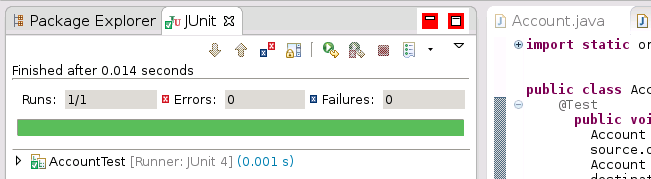
\includegraphics[width=.6\textwidth]{L02/pass}
\end{center}
  
Writing self-checking tests means that the tests automatically report
the status of the code. This enables a ``keep the bar green'' coding
style. Implications: 1) you can worry less about introducing bugs (but
still take ordinary care); and 2) the tests help document your
system's specs.

\paragraph{How to write self-checking tests.}
One might think:
\begin{quote}
  ``Isn't it just calling asserts?''
\end{quote}

Sadly, no. That's not enough.

Two questions about actually deploying asserts:
\begin{itemize}[noitemsep]
\item Q: what for?\\
  A: check method call results
\item Q: where?\\
  A: usually after calling SUT (System Under Test)
\end{itemize}

\paragraph{Counter example.} Here's some example code.
\codelisting{}{L02/Counter.java}
We can test it with the following JUnit test.
\codelisting{}{L02/CounterTest.java}

What kind of test is this? Let's consider two kinds of
tests: state-based tests vs. behaviour-based tests.

\begin{itemize}[noitemsep]
\item {\bf State:} e.g. object field values.
    Verify by calling accessor methods.
  \item {\bf Behaviour:} which calls SUT makes.
    Verify by inserting observation points, monitoring interactions.
\end{itemize}

Does Counter Test verify state or behaviour?

\paragraph{Flight example.} Here's more example code.
\codelisting{}{L02/flight.java}

\newpage
\subsection*{Implementing State Verification}
We can verify state:
\codelisting{}{L02/flight_extended_state_spec.java}

Note that we are exercising the SUT, verifying state,
and checking return values.

In state-based tests, we inspect only outputs, and only call methods from SUT. We do not instrument the SUT. We do not check interactions.

You have two options for verifying state:
\begin{enumerate}[noitemsep]
\item procedural (bunch of asserts); or,
\item via expected objects (won't talk about them this year).
\end{enumerate}

Returning to the flight example:
\begin{itemize}[noitemsep]
\item We do check that the flight got removed.
\item We don't check that the removal got logged.
\item Hard to check state and observe logging.
\item Solution: Spy on SUT behaviour.
\end{itemize}

\newpage
\subsection*{Implementing Procedural Behaviour Verification}
Or, we can implement behaviour verification. This is one
way to do so, behaviourally:
\codelisting{}{L02/flight_pbv.java}

As an alternative, we can use a mock object framework (e.g. JMock) to
define expected behaviour.

\paragraph{Idea.} Observe calls to the logger,
make sure right calls happen.

\subsection*{Assertions}
We build tests using assertions. 
In JUnit, there are three basic built-in choices:
\begin{enumerate}[noitemsep]
\item assertTrue(aBooleanExpression)
\item assertEquals(expected, actual)
\item assertEquals(expected, actual, tolerance)
\end{enumerate}
(There are others too, but let's start with these.)

{\tt assertTrue} is more flexible, since you can
write anything with a boolean value. However, it can give
hard-to-diagnose error messages---you need try harder when using it
if you want good tests.

\paragraph{Using Assertions.}
Why use assertions? Assertions are good for:
\begin{itemize}[noitemsep]
\item checking all the things that should be true (more = better);
\item serving as documentation:
    when system in state $S_1$,
    and I do $X$,
    assert that the result should be $R$, and
    that system should be in $S_2$.
\item allowing failure diagnosis (include assertion messages!)
\end{itemize}

\newpage
There are alternatives to using assertions.
For instance, one can also do external result verification:
\begin{itemize}[noitemsep]
\item write output to files; and
\item use diff (or your own custom diff) to compare
  expected and actual output.
\end{itemize}

The twist is that the expected result is then not visible when looking
at test's source code. (What's a good workaround?)

\paragraph{Verifying Behaviour.} The key is to observe actions
(calls) of the SUT. Some options:
\begin{itemize}[noitemsep]
\item procedural behaviour verification
  (the challenge in that case: recording and verifying behaviour); or
\item expected behaviour specification
  (capturing the outbound calls of the SUT).
\end{itemize}

\section*{Test Doubles}
Mock objects are a particular kind of test double. We need test doubles
because objects collaborate with other objects, but we only want to test
one object at a time.
Meszaros categorizes test doubles as follows:
\begin{itemize}[noitemsep]
    \item dummy objects: these are not actually test doubles; they don't do anything, but just take up space in parameter lists. Are like {\tt null}, but get past nullness checks in code.
    \item fake objects: have actual behaviour (which is correct), but somehow unsuitable for use in production; typical example is an in-memory database.
    \item stubs: produce canned answers in response to interactions from the class under test.
    \item mocks: like stubs, also produce canned answers. Difference: mock objects also check that the class under test makes the appropriate calls.
    \item spies: usually wraps the real object (instead of the mock, which stubs it), and records interactions for later verification.
\end{itemize}
Shorter reference about test doubles: \url{martinfowler.com/articles/mocksArentStubs.html}

\section*{Mock Objects}
Before we talk about mock objects, let's look at a stub. Imagine that you have a service that
sends out emails. You don't actually want to send out emails while you're testing. So here's
a class that pretends to send out emails.
\codelisting{}{L02/MailServiceStub.java}
This stub permits \emph{state verification}, as seen in the following assert in a test:
\begin{lstlisting}
  assertEquals(1, mailer.numberSent());
\end{lstlisting}
This is state verification because it's checking the contents of
memory (which should reflect interactions that have happened in the
past). One could also check the recipients, contents of messages, etc.

\paragraph{jMock example.} 
Instead of state verification, we can also do behaviour verification. This is
jMock syntax.
\codelisting{}{L02/OrderInteractionTester.java}
The calls to {\tt mock()} create mock objects which have the
appropriate type.  If you are using the objects as simple dummy
objects, calling {\tt mock()} and {\tt proxy()} is enough. Note that
we have a real {\tt Order} object but we're giving it the fake proxy
objects, as created by the {\tt Mock}'s {\tt proxy()} methods.

We also specify the expected behaviour of the {\tt mailer} and the
{\tt warehouse}. The test case is saying that the mailer ought to have
{\tt send()} called on it once, and that the warehouse ought to have
{\tt hasInventory()} called; that method should return {\tt false()}.

\paragraph{EasyMock example.} Different mock object libraries have different syntax. Here's 
another example, this time for EasyMock.

\codelisting{}{L02/ExampleTest.java}
Here we are testing the {\tt ClassUnderTest} and creating a mock object
of {\tt Collaborator} type. EasyMock 2.3 reads the {\tt @Mock} annotation
and automatically fills in a mock object of the appropriate type.
In our test case, we call {\tt replay(mock)} to indicate that we are no
longer recording expectations, but are instead starting the test case itself.
In the above code, there are currently no expectations.

Let's add some expectations.
\codelisting{}{L02/TestAddDocument.java}
Here we record the fact that the mock should be called with {\tt documentAdded}
and a parameter "New Document". We also record that the mock's 
{\tt voteForRemoval} method should be called, and when that happens, it should return
value 42.
Finally, we add a call {\tt verify()} to let EasyMock
know that we're done and that it can go ahead and check that the expected behaviour actually happened.

\section*{Flaky Tests}
The second test engineering topic I want to talk about today is flaky tests. 
Flaky tests are those that sometimes fail (nondeterministically).
Flakiness is not something you want in your test cases. 
(I have heard one defense of a flaky test: it lets you know that 
the system has the potential to actually work.) 
In general, flaky tests don't play well with the expectation that
your test suite passes 100\%.

Reference:\\
Qingzhou Luo, Farah Hariri, Lamyaa Eloussi, Darko Marinov. ``An Empirical Analysis of Flaky Tests''. In Proceedings of Foundations of Software Engineering '14.

\paragraph{Dealing with flaky tests.} Companies with large test suites have found mitigations
for the flaky test suite problem. One can label known-flaky tests as flaky and automatically
re-run them to see if they eventually pass. One can also ignore or remove flaky tests.
But this is unsatisfactory: it takes a long time to re-run failing tests.

\paragraph{Causes of flakiness.} Luo et al studied 201 fixes to flaky tests in open-source
projects. They found that the three most common causes of fixable flaky tests were:
\begin{enumerate}[noitemsep]
    \item improper waits for asynchronous responses;
    \item concurrency; and
    \item test order dependency.
\end{enumerate}

The problem that caused flakiness for asynchronous waits was that there was typically a
{\tt sleep()} call which didn't wait long enough for the action (perhaps a network call)
to finish. The best practice is to use some sort of {\tt wait()} call to wait for the result
instead of hardcoding a sleep time.

Concurrency problems were what one might expect. The problem could either be in the system under
test or in the test itself. Problems included data races, atomicity violations, and deadlocks;
the solutions were the proper use of concurrency primitives (e.g. locks) as seen in CS343.

Test order dependency problems arose when some tests expected other tests to have already
executed (and left a side effect like a file in the filesystem). They came up especially 
in the transition from Java 6 to Java 7 because that transition changed the (not-guaranteed)
test execution order. The solution is to remove the dependency.

\section*{Not unit tests}
Many interesting things happen when different units interact.
Integration tests verify end-to-end functionality. They're slower, flakier, and harder both
to write and use. Focus on unit tests while developing code. But you eventually need
integration tests to make sure the user sees the right thing.




% L23, L24 from old notes

\end{document}
